% 三角形三色問題の概要(数学)
% 調和彩色三角形 (well-colored triangle)
% 三色三角形が調和している
% 三色三角形が調和性をみたす
\section{三角形三色問題の概要}
三角形三色問題について述べる前に調和性の定義と調和彩色三角形の定義について先に述べる.
\begin{dfn}[調和性] \label{dfn:wc}
  $3$つのマスに塗られている色がすべて同じか相異なるとき,この$3$マスは調和性を満たす,
  または,調和しているという.
\end{dfn}

\begin{exm}
  図$\ref{wellcoloed}$のような$3$マスの組は調和性を満たしているが,
  図$\ref{notwellcoloed}$のような$3$マスの組は調和性を満たしていない.
  \begin{figure}[h]
    \centering
    % wellcolored
\begin{tikzpicture}[scale=0.25]
  % 左図
  \begin{scope}[xshift={-150}]
    \myHexB{-1}{1}
    \myHexY{1}{1}
    \myHexR{0}{0}
  \end{scope}
  % 右図  
  \begin{scope}[xshift={150}]
    \myHexY{-1}{1}
    \myHexY{1}{1}
    \myHexY{0}{0}
  \end{scope}
\end{tikzpicture}

    \caption{調和性を満たす$3$色の組}
    \label{wellcoloed}
  \end{figure}
  \begin{figure}[h]
    \centering
    % wellcolored
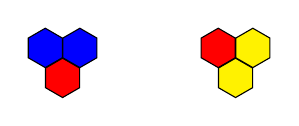
\begin{tikzpicture}[scale=0.25]
  %1段目
  \filldraw[fill=red,xshift={-25*5},yshift={25*sqrt(3)*3}] (0,0)--++(30:1)--++(90:1)--++(150:1)--++(210:1)--++(270:1)--cycle;
  \filldraw[fill=yellow,xshift={25*5},yshift={25*sqrt(3)*3}] (0,0)--++(30:1)--++(90:1)--++(150:1)--++(210:1)--++(270:1)--cycle;
  %0段目
  \filldraw[fill=blue,xshift={-25*4},yshift={25*sqrt(3)*4}] (0,0)--++(30:1)--++(90:1)--++(150:1)--++(210:1)--++(270:1)--cycle;
  \filldraw[fill=blue,xshift={-25*6},yshift={25*sqrt(3)*4}] (0,0)--++(30:1)--++(90:1)--++(150:1)--++(210:1)--++(270:1)--cycle;
  \filldraw[fill=yellow,xshift={25*6},yshift={25*sqrt(3)*4}] (0,0)--++(30:1)--++(90:1)--++(150:1)--++(210:1)--++(270:1)--cycle;
  \filldraw[fill=red,xshift={25*4},yshift={25*sqrt(3)*4}] (0,0)--++(30:1)--++(90:1)--++(150:1)--++(210:1)--++(270:1)--cycle;
\end{tikzpicture}

    \caption{調和性を満たさない$3$色の組}
    \label{notwellcoloed}
  \end{figure}
\end{exm}

次に三角形三色問題について述べる.
$n(>0)$段
\footnote{
  先述の通り段数の数え方は 0 段目, 1 段目, 2 段目,... である.
  }
の逆三角形に配置された六角形のマスがある.
最上段のそれぞれのマスには$3$色(赤,黄,青)のうち1色がランダムに塗られており,
次の規則に従って上から下へ$3$色(赤,黄,青)を用いて塗る.
規則は次の$2$つである.
\begin{itemize}
  \item
    隣り合う$2$つのマスの色が同じとき,同じ色を間にある$1$段下のマスに塗る.
  \item
    隣り合う$2$つのマスの色が異なるとき,どちらとも違う第三の色を間にある$1$段下のマスに塗る.
\end{itemize}
すなわち,逆三角形の隣接する$3$つのマスはすべて調和性を満たすように色を塗る.
図\ref{fig:nine_steps}は$n=9$のときに規則に従って3色で塗った三色三角形である.
このとき,最下段のマスの色は赤であり,最上段の両端のマスは黄,青であるから
最上段の両端のマスの色と最下段のマスの色について調和性を満たしていることが分かる.
\begin{figure}[h]
    \centering
    % 9steps
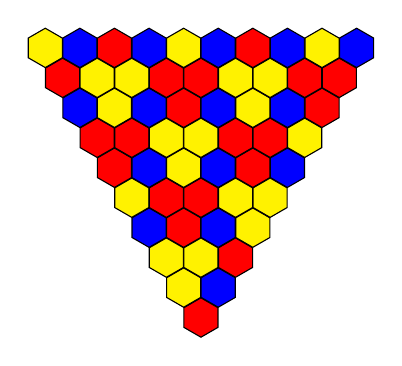
\begin{tikzpicture}[scale=0.25]
  %9段目
  \filldraw[fill=red] (0,0)--++(30:1)--++(90:1)--++(150:1)--++(210:1)--++(270:1)--cycle;
  %8段目
  \filldraw[fill=yellow,xshift={-25},yshift={25*sqrt(3)}] (0,0)--++(30:1)--++(90:1)--++(150:1)--++(210:1)--++(270:1)--cycle;
  \filldraw[fill=blue,xshift={25},yshift={25*sqrt(3)}] (0,0)--++(30:1)--++(90:1)--++(150:1)--++(210:1)--++(270:1)--cycle;
  %7段目
  \filldraw[fill=yellow,xshift={-25*2},yshift={25*sqrt(3)*2}] (0,0)--++(30:1)--++(90:1)--++(150:1)--++(210:1)--++(270:1)--cycle;
  \filldraw[fill=yellow,yshift={25*sqrt(3)*2}] (0,0)--++(30:1)--++(90:1)--++(150:1)--++(210:1)--++(270:1)--cycle;
  \filldraw[fill=red,xshift={25*2},yshift={25*sqrt(3)*2}] (0,0)--++(30:1)--++(90:1)--++(150:1)--++(210:1)--++(270:1)--cycle;
  %6段目
  \filldraw[fill=blue,xshift={-25*3},yshift={25*sqrt(3)*3}] (0,0)--++(30:1)--++(90:1)--++(150:1)--++(210:1)--++(270:1)--cycle;
  \filldraw[fill=red,xshift={-25},yshift={25*sqrt(3)*3}] (0,0)--++(30:1)--++(90:1)--++(150:1)--++(210:1)--++(270:1)--cycle;
  \filldraw[fill=blue,xshift={25},yshift={25*sqrt(3)*3}] (0,0)--++(30:1)--++(90:1)--++(150:1)--++(210:1)--++(270:1)--cycle;
  \filldraw[fill=yellow,xshift={25*3},yshift={25*sqrt(3)*3}] (0,0)--++(30:1)--++(90:1)--++(150:1)--++(210:1)--++(270:1)--cycle;
  %5段目
  \filldraw[fill=yellow,xshift={-25*4},yshift={25*sqrt(3)*4}] (0,0)--++(30:1)--++(90:1)--++(150:1)--++(210:1)--++(270:1)--cycle;
  \filldraw[fill=red,xshift={-25*2},yshift={25*sqrt(3)*4}] (0,0)--++(30:1)--++(90:1)--++(150:1)--++(210:1)--++(270:1)--cycle;
  \filldraw[fill=red,yshift={25*sqrt(3)*4}] (0,0)--++(30:1)--++(90:1)--++(150:1)--++(210:1)--++(270:1)--cycle;
  \filldraw[fill=yellow,xshift={25*2},yshift={25*sqrt(3)*4}] (0,0)--++(30:1)--++(90:1)--++(150:1)--++(210:1)--++(270:1)--cycle;
  \filldraw[fill=yellow,xshift={25*4},yshift={25*sqrt(3)*4}] (0,0)--++(30:1)--++(90:1)--++(150:1)--++(210:1)--++(270:1)--cycle;
  %4段目
  \filldraw[fill=red,xshift={-25*5},yshift={25*sqrt(3)*5}] (0,0)--++(30:1)--++(90:1)--++(150:1)--++(210:1)--++(270:1)--cycle;
  \filldraw[fill=blue,xshift={-25*3},yshift={25*sqrt(3)*5}] (0,0)--++(30:1)--++(90:1)--++(150:1)--++(210:1)--++(270:1)--cycle;
  \filldraw[fill=yellow,xshift={-25*1},yshift={25*sqrt(3)*5}] (0,0)--++(30:1)--++(90:1)--++(150:1)--++(210:1)--++(270:1)--cycle;
  \filldraw[fill=blue,xshift={25*1},yshift={25*sqrt(3)*5}] (0,0)--++(30:1)--++(90:1)--++(150:1)--++(210:1)--++(270:1)--cycle;
  \filldraw[fill=red,xshift={25*3},yshift={25*sqrt(3)*5}] (0,0)--++(30:1)--++(90:1)--++(150:1)--++(210:1)--++(270:1)--cycle;
  \filldraw[fill=blue,xshift={25*5},yshift={25*sqrt(3)*5}] (0,0)--++(30:1)--++(90:1)--++(150:1)--++(210:1)--++(270:1)--cycle;
  %3段目
  \filldraw[fill=red,xshift={-25*6},yshift={25*sqrt(3)*6}] (0,0)--++(30:1)--++(90:1)--++(150:1)--++(210:1)--++(270:1)--cycle;
  \filldraw[fill=red,xshift={-25*4},yshift={25*sqrt(3)*6}] (0,0)--++(30:1)--++(90:1)--++(150:1)--++(210:1)--++(270:1)--cycle;
  \filldraw[fill=yellow,xshift={-25*2},yshift={25*sqrt(3)*6}] (0,0)--++(30:1)--++(90:1)--++(150:1)--++(210:1)--++(270:1)--cycle;
  \filldraw[fill=yellow,yshift={25*sqrt(3)*6}] (0,0)--++(30:1)--++(90:1)--++(150:1)--++(210:1)--++(270:1)--cycle;
  \filldraw[fill=red,xshift={25*2},yshift={25*sqrt(3)*6}] (0,0)--++(30:1)--++(90:1)--++(150:1)--++(210:1)--++(270:1)--cycle;
  \filldraw[fill=red,xshift={25*4},yshift={25*sqrt(3)*6}] (0,0)--++(30:1)--++(90:1)--++(150:1)--++(210:1)--++(270:1)--cycle;
  \filldraw[fill=yellow,xshift={25*6},yshift={25*sqrt(3)*6}] (0,0)--++(30:1)--++(90:1)--++(150:1)--++(210:1)--++(270:1)--cycle;
  %2段目
  \filldraw[fill=blue,xshift={-25*7},yshift={25*sqrt(3)*7}] (0,0)--++(30:1)--++(90:1)--++(150:1)--++(210:1)--++(270:1)--cycle;
  \filldraw[fill=yellow,xshift={-25*5},yshift={25*sqrt(3)*7}] (0,0)--++(30:1)--++(90:1)--++(150:1)--++(210:1)--++(270:1)--cycle;
  \filldraw[fill=blue,xshift={-25*3},yshift={25*sqrt(3)*7}] (0,0)--++(30:1)--++(90:1)--++(150:1)--++(210:1)--++(270:1)--cycle;
  \filldraw[fill=red,xshift={-25*1},yshift={25*sqrt(3)*7}] (0,0)--++(30:1)--++(90:1)--++(150:1)--++(210:1)--++(270:1)--cycle;
  \filldraw[fill=blue,xshift={25*1},yshift={25*sqrt(3)*7}] (0,0)--++(30:1)--++(90:1)--++(150:1)--++(210:1)--++(270:1)--cycle;
  \filldraw[fill=yellow,xshift={25*3},yshift={25*sqrt(3)*7}] (0,0)--++(30:1)--++(90:1)--++(150:1)--++(210:1)--++(270:1)--cycle;
  \filldraw[fill=blue,xshift={25*5},yshift={25*sqrt(3)*7}] (0,0)--++(30:1)--++(90:1)--++(150:1)--++(210:1)--++(270:1)--cycle;
  \filldraw[fill=red,xshift={25*7},yshift={25*sqrt(3)*7}] (0,0)--++(30:1)--++(90:1)--++(150:1)--++(210:1)--++(270:1)--cycle;
  %1段目
  \filldraw[fill=red,xshift={-25*8},yshift={25*sqrt(3)*8}] (0,0)--++(30:1)--++(90:1)--++(150:1)--++(210:1)--++(270:1)--cycle;
  \filldraw[fill=yellow,xshift={-25*6},yshift={25*sqrt(3)*8}] (0,0)--++(30:1)--++(90:1)--++(150:1)--++(210:1)--++(270:1)--cycle;
  \filldraw[fill=yellow,xshift={-25*4},yshift={25*sqrt(3)*8}] (0,0)--++(30:1)--++(90:1)--++(150:1)--++(210:1)--++(270:1)--cycle;
  \filldraw[fill=red,xshift={-25*2},yshift={25*sqrt(3)*8}] (0,0)--++(30:1)--++(90:1)--++(150:1)--++(210:1)--++(270:1)--cycle;
  \filldraw[fill=red,yshift={25*sqrt(3)*8}] (0,0)--++(30:1)--++(90:1)--++(150:1)--++(210:1)--++(270:1)--cycle;
  \filldraw[fill=yellow,xshift={25*2},yshift={25*sqrt(3)*8}] (0,0)--++(30:1)--++(90:1)--++(150:1)--++(210:1)--++(270:1)--cycle;
  \filldraw[fill=yellow,xshift={25*4},yshift={25*sqrt(3)*8}] (0,0)--++(30:1)--++(90:1)--++(150:1)--++(210:1)--++(270:1)--cycle;
  \filldraw[fill=red,xshift={25*6},yshift={25*sqrt(3)*8}] (0,0)--++(30:1)--++(90:1)--++(150:1)--++(210:1)--++(270:1)--cycle;
  \filldraw[fill=red,xshift={25*8},yshift={25*sqrt(3)*8}] (0,0)--++(30:1)--++(90:1)--++(150:1)--++(210:1)--++(270:1)--cycle;
  %0段目
  \filldraw[fill=yellow,xshift={-25*9},yshift={25*sqrt(3)*9}] (0,0)--++(30:1)--++(90:1)--++(150:1)--++(210:1)--++(270:1)--cycle;
  \filldraw[fill=blue,xshift={-25*7},yshift={25*sqrt(3)*9}] (0,0)--++(30:1)--++(90:1)--++(150:1)--++(210:1)--++(270:1)--cycle;
  \filldraw[fill=red,xshift={-25*5},yshift={25*sqrt(3)*9}] (0,0)--++(30:1)--++(90:1)--++(150:1)--++(210:1)--++(270:1)--cycle;
  \filldraw[fill=blue,xshift={-25*3},yshift={25*sqrt(3)*9}] (0,0)--++(30:1)--++(90:1)--++(150:1)--++(210:1)--++(270:1)--cycle;
  \filldraw[fill=yellow,xshift={-25*1},yshift={25*sqrt(3)*9}] (0,0)--++(30:1)--++(90:1)--++(150:1)--++(210:1)--++(270:1)--cycle;
  \filldraw[fill=blue,xshift={25*1},yshift={25*sqrt(3)*9}] (0,0)--++(30:1)--++(90:1)--++(150:1)--++(210:1)--++(270:1)--cycle;
  \filldraw[fill=red,xshift={25*3},yshift={25*sqrt(3)*9}] (0,0)--++(30:1)--++(90:1)--++(150:1)--++(210:1)--++(270:1)--cycle;
  \filldraw[fill=blue,xshift={25*5},yshift={25*sqrt(3)*9}] (0,0)--++(30:1)--++(90:1)--++(150:1)--++(210:1)--++(270:1)--cycle;
  \filldraw[fill=yellow,xshift={25*7},yshift={25*sqrt(3)*9}] (0,0)--++(30:1)--++(90:1)--++(150:1)--++(210:1)--++(270:1)--cycle;
  \filldraw[fill=blue,xshift={25*9},yshift={25*sqrt(3)*9}] (0,0)--++(30:1)--++(90:1)--++(150:1)--++(210:1)--++(270:1)--cycle;
\end{tikzpicture}

    \caption{三色三角形($n=9$のとき)}
    \label{fig:nine_steps}
\end{figure}
$n=9$の場合は図\ref{fig:nine_steps}の塗り方でなくとも逆三角形の$3$つの頂点のマスは調和性を満たすことが観察できる.

このことから次のような仮説が考えられる.
\begin{itemize}
  \item[(仮説)]
  最上段をどのように塗っても最上段の両端のマスの色と最下段のマスの色は調和性を満たす.
\end{itemize}

数学セミナー誌で出題された三角形三色問題は次の$2$つの問題のことである~\cite{Nishiyama2}.
\begin{enumerate}
\item \label{que:1}
  $n=9$のとき仮説が成立することを証明せよ.
\item \label{que:2}
  $n=9$以外に仮説が成立する段数が存在するか調べ,存在するならば$n$の一般式を求めよ.
\end{enumerate}

この問題については既に解答が得られており,
一般に$n=3^k$段の逆三角形において仮説が成立することを示す次の定理が示されている.

\begin{dfn}[調和彩色三角形] \label{dfn:wc_tri}
  $3$つの端点のマスに塗られている色が調和性を満たしている三色三角形を調和彩色三角形 $(well-colored triangle)$ という.
\end{dfn}

\begin{thm} \label{thm:tri_iff}
  $n(>0)$段の逆三角形に配置されたマス対して,
  最上段のマスを$3$色で任意に塗った後,規則に従って残りのマスに色を塗ったとき
  \[
  (\exists k.n=3^k) \Leftrightarrow \text{$n$段の逆三角形は常に調和彩色三角形}.
  \]
\end{thm}

本節ではこの定理の証明を Coq で実装するにあたり,証明の概要について述べる.

% 2.1 n=3^k => 調和三角形
\subsection{十分条件}
定理\ref{thm:tri_iff}を証明するにあたって,十分条件と必要条件に分けて話を進める.
ここでは定理\ref{thm:tri_iff}の十分条件である補題\ref{lem:tri_suf}の証明の概要について述べる.
\begin{lem}[十分条件] \label{lem:tri_suf}
  $n$ 段の逆三角形に配置されたマス対して,
  最上段のマスを$3$色で任意に塗った後,規則に従って残りのマスに色を塗ったとき
  \[
  (\exists k.n=3^k) \Imp \text{$n$段の逆三角形は常に調和彩色三角形}.
  \]
\end{lem}
補題\ref{lem:tri_suf}を証明するためには論理同値である次の命題を証明すればよい.
\[
\forall k.(n=3^k \Imp \text{$n$段の逆三角形は常に調和彩色三角形}).
\]
これは$k$に関する数学的帰納法を用いて証明する.
\begin{itemize}
\item
  $k=0$のときは$n=1$となり明らかに成立する.
\item
  $k$ のとき成立すると仮定する.
すなわち,$3^{k}$段の三色三角形ならば常に調和彩色三角形であると仮定する.
ここで各マスに塗られている色を図\ref{fig:ind_steps}のように表す.
ただし,図中の$c^x_y$ は左から$x$個目,上から$y$段目のマスに塗られている色を表している.
\begin{figure}[h]
    \centering
    % 3^{k+1} 段の三角形
\begin{tikzpicture}
  {\footnotesize{
      % 3^(k+1)段目
      \node (a0) {$c^{0}_{3^{k+1}}$};
      % 2*3^k段目
      \node[above left=0.2cm of a0] (b0) {$c^{0}_{2\cdot3^{k}}$};
      \node[above right=0.2cm of a0] (b1) {$c^{3^{k}}_{2\cdot3^{k}}$};
      % 3^k段目
      \node[above left=0.25cm of b0] (c0) {$c^{0}_{3^{k}}$};
      \node[above right=0.25cm of b0] (c1) {$c^{3^{k}}_{3^{k}}$};
      \node[above right=0.1cm of b1] (c2) {$c^{2\cdot3^{k}}_{3^{k}}$};
      % 0段目
      \node[above left=0.3cm of c0] (d0) {$c^{0}_{0}$};
      \node[above right=0.3cm of c0] (d1) {$c^{3^{k}}_{0}$};
      \node[above left=0.1cm of c2] (d2) {$c^{2\cdot3^{k}}_{0}$};
      \node[above right=0.1cm of c2] (d3) {$c^{3^{k+1}}_{0}$};
      % 点線 [3^(k+1)段 〜 2*3^k 段]
      \node[blue] at ($(a0)!.5!(b0)$) {$\ddots$};
      \node[blue] at ($(b0)!.5!(b1)$) {$\cdots$};
      \node[blue] at ($(a0)!.5!(b1)$) {$\iddots$};
      % 点線 [2*3^k 段 〜 3^k 段]
      \node[teal] at ($(b0)!.5!(c0)$) {$\ddots$};
      \node[teal] at ($(c0)!.5!(c1)$) {$\cdots$};
      \node[teal] at ($(b0)!.5!(c1)$) {$\iddots$};
      \node[red] at ($(b1)!.5!(c1)$) {$\ddots$};
      \node[red] at ($(c1)!.5!(c2)$) {$\cdots$};
      \node[red] at ($(b1)!.5!(c2)$) {$\iddots$};
      % 点線 [3^k 段 〜 0 段]
      \node[red] at ($(c0)!.5!(d0)$) {$\ddots$};
      \node[red] at ($(d0)!.5!(d1)$) {$\cdots$};
      \node[red] at ($(c0)!.5!(d1)$) {$\iddots$};
      \node[blue] at ($(c1)!.5!(d1)$) {$\ddots$};
      \node[blue] at ($(d1)!.5!(d2)$) {$\cdots$};
      \node[blue] at ($(c1)!.5!(d2)$) {$\iddots$};
      \node[teal] at ($(c2)!.5!(d2)$) {$\ddots$};
      \node[teal] at ($(d2)!.5!(d3)$) {$\cdots$};
      \node[teal] at ($(c2)!.5!(d3)$) {$\iddots$};
  }}
\end{tikzpicture}

    \caption{三色三角形($n=3^{k+1}$のとき)}
    \label{fig:ind_steps}
\end{figure} 
ここで,図\ref{fig:ind_steps}の中にある$3^k$段の逆三角形に注目する.
注目する逆三角形を$3$つ端点のマスの色を組にして表すことにすると,
上から$0$段目から$3^{k}$段目の間にある逆三角形は次の$3$個である.
\[
\left(c^{0}_{0},c^{3^{k}}_{0},c^{0}_{3^{k}}\right),
\quad
\left(c^{3^{k}}_{0},c^{2\cdot3^{k}}_{0},c^{3^{k}}_{3^{k}}\right),
\]
\[
\left(c^{2\cdot3^{k}}_{0},c^{3^{k+1}}_{0},c^{2\cdot3^{k}}_{3^{k}}\right).
\]
また,上から$3^{k}$段目から$2\cdot3^{k}$段目の間にある逆三角形は次の$2$個である.
\[
\left(c^{0}_{3^{k}},c^{3^{k}}_{3^{k}},c^{0}_{2\cdot3^{k}}\right),
\quad
\left(c^{3^{k}}_{3^{k}},c^{2\cdot3^{k}}_{3^{k}},c^{3^{k}}_{2\cdot3^{k}}\right).
\]
さらに,上から$2\cdot3^{k}$段目から$3^{k+1}$段目の間にある逆三角形は次の$1$個である.
\[
\left(c^{0}_{2\cdot3^{k}},c^{3^{k}}_{2\cdot3^{k}},c^{0}_{3^{k+1}}\right).
\]
これらの$6$個の$3^k$段の逆三角形はすべて帰納法の仮定により常に調和彩色三角形である.
よって,調和彩色三角形の定義より最上段のマスの$4$色$c^0_0, c^{3^{k}}_0, c^{2\cdot3^{k}}_0, c^{3^{k+1}}_0$から最下段のマスの$c^0_{3^{k+1}}$の色が得られる.
さらにこのとき,最上段のマスの$4$色$c^0_0, c^{3^{k}}_0, c^{2\cdot3^{k}}_0, c^{3^{k+1}}_0$から得られた色$c^0_{3^{k+1}}$は$2$色$c^0_0, c^{3^{k+1}}_0$のみからでも得られる.
これは色の場合分けをすることで証明できるが,詳細は補題\ref{lem:mixCut}で述べる.
したがって,最上段の両端のマスに塗られている色$c^0_0, c^{3^{k+1}}_0$から規則に従うことで最下段の色$c^0_{3^{k+1}}$を得られるので調和性を満たす.
すなわち,$3^{k+1}$段の逆三角形は常に調和彩色三角形である.
\end{itemize}

% 2.2 調和 (well-colored) => n=3^k
\subsection{必要条件}
次は定理\ref{thm:tri_iff}の必要条件である補題\ref{lem:tri_nec}の証明の概要について述べる.
\begin{lem}[必要条件] \label{lem:tri_nec}
  $n(>0)$段の逆三角形に配置されたマス対して,
  最上段のマスを$3$色で任意に塗った後,規則に従って残りのマスに色を塗ったとき
  \[
  \text{$n$段の逆三角形は常に調和彩色三角形} \Imp (\exists k.n=3^k).
  \]
\end{lem}
補題\ref{lem:tri_nec}の証明では対偶法を用いた後に,$n$に関する場合分けをして証明する.
補題\ref{lem:tri_nec}の対偶は以下の通り.

$\lnot$ $(\exists$ $k.n=3^k)$ $\Imp$ $\lnot($ $n$段の逆三角形は常に調和彩色三角形$)$.

したがって,$\lnot(\exists k.n=3^k)$を仮定したとき,次の各場合について調和彩色三角形にならない最上段のマスの塗り方を挙げればよい.
場合分けの仕方は次の$3$つである.
\begin{enumerate}
\item \label{case:even}
  $n$が偶数
\item \label{case:shortodd}
  $n$が奇数 かつ $3^{k} < n \leq 2 \cdot 3^{k}$
\item \label{case:longodd}
  $n$が奇数 かつ $2 \cdot 3^{k} + 1 \leq n < 3^{k+1}$
\end{enumerate}
各場合について調和彩色三角形にならないような最上段のマスの塗り方は次の通り.
\begin{itemize}
  \item
    \ref{case:even}.のときは最上段のマスを黄,青の順で交互に塗る.
    すると,黄,青を交互に塗られているので第$1$段目のマスは規則よりすべて赤色で塗られている.
    さらに,規則より最下段のマスまですべて赤で塗られている.
    したがって,$n$が偶数であるから最上段の両端のマスは黄であり,最下段のマスの色が赤であるから調和性を満たさないので調和彩色三角形でない.
    \begin{figure}[h]
      \centering
      % even_steps
\begin{tikzpicture}[scale=0.25]
  %3^(k'+1)段目
  \myHexR{0}{0}
  %2 〜 3^(K'+1)-1段目
  \node[xshift={-25*1},yshift={25*sqrt(3)*0.6}](0,0){$\ddots$};
  \node[xshift={25*1},yshift={25*sqrt(3)*0.6}](0,0){$\iddots$};
  %1段目
  \myHexR{-7}{3}
  \myHexR{-5}{3}  
  \node[yshift={25*sqrt(3)*0.9}](0,0){$\cdots$};
  \myHexR{5}{3}
  \myHexR{7}{3}
  %0段目
  \myHexY{-8}{4}
  \myHexB{-6}{4}
  \myHexY{-4}{4}  
  \node[yshift={25*sqrt(3)*1.2}](0,0){$\cdots$};
  \myHexY{4}{4}
  \myHexB{6}{4}
  \myHexY{8}{4}  
\end{tikzpicture}

      \caption{$n$が偶数}
      \label{fig:even_steps}
    \end{figure}
  \item
    \ref{case:shortodd}.のときは最上段のマスを外側の両端のマスから内側の方に向かって黄,青の順で$2$色を用いて対称的に交互に塗る.
    すると,補題\ref{lem:tri_suf}より最上段から$3^k$段下のマスは調和彩色三角形の定義より黄,青の順で交互に塗られている.
    これは\ref{case:even}.の場合に帰着できるので最下段のマスの色は赤である.
    したがって,最上段の両端のマスの色は黄であり,最下段のマスの色が赤であるから調和性を満たさないので調和彩色三角形でない.
    \begin{figure}[h]
      \centering
      % oddshort_steps
\definecolor{grayR}{rgb}{0.50, 0.50, 0.50}
\definecolor{grayB}{rgb}{0.10, 0.10, 0.10}
\definecolor{grayY}{rgb}{1.00, 1.00, 1.00}
%\def\myRed{red}
%\def\myBlue{blue}
%\def\myYellow{yellow}
\def\myRed{grayR}
\def\myBlue{grayB}
\def\myYellow{grayY}

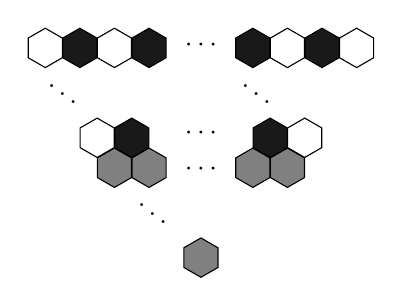
\begin{tikzpicture}[scale=0.25]
  %3^(k'+1)段目
  \filldraw[fill=\myRed,yshift={25*sqrt(3)*2}] (0,0)--++(30:1)--++(90:1)--++(150:1)--++(210:1)--++(270:1)--cycle;
  %3^k'+2 〜 3^(k'+1)-1段目
  \node[yshift={25*sqrt(3)*1.4}](0,0){$\cdots$};
  \node[xshift={-25*0.7},yshift={25*sqrt(3)*1.1}](0,0){$\ddots$};
  \node[xshift={25*0.7},yshift={25*sqrt(3)*1.1}](0,0){$\iddots$};
  %3^k'+1段目
  \filldraw[fill=\myRed,xshift={-25*5},yshift={25*sqrt(3)*5}] (0,0)--++(30:1)--++(90:1)--++(150:1)--++(210:1)--++(270:1)--cycle;
  \filldraw[fill=\myRed,xshift={-25*3},yshift={25*sqrt(3)*5}] (0,0)--++(30:1)--++(90:1)--++(150:1)--++(210:1)--++(270:1)--cycle;
  \node[yshift={25*sqrt(3)*1.7}](0,0){$\cdots$};
  \filldraw[fill=\myRed,xshift={25*3},yshift={25*sqrt(3)*5}] (0,0)--++(30:1)--++(90:1)--++(150:1)--++(210:1)--++(270:1)--cycle;
  \filldraw[fill=\myRed,xshift={25*5},yshift={25*sqrt(3)*5}] (0,0)--++(30:1)--++(90:1)--++(150:1)--++(210:1)--++(270:1)--cycle;
  %3^k'段目
  \filldraw[fill=\myYellow,xshift={-25*6},yshift={25*sqrt(3)*6}] (0,0)--++(30:1)--++(90:1)--++(150:1)--++(210:1)--++(270:1)--cycle;
  \filldraw[fill=\myBlue,xshift={-25*4},yshift={25*sqrt(3)*6}] (0,0)--++(30:1)--++(90:1)--++(150:1)--++(210:1)--++(270:1)--cycle;
  \filldraw[fill=\myBlue,xshift={25*4},yshift={25*sqrt(3)*6}] (0,0)--++(30:1)--++(90:1)--++(150:1)--++(210:1)--++(270:1)--cycle;
  \filldraw[fill=\myYellow,xshift={25*6},yshift={25*sqrt(3)*6}] (0,0)--++(30:1)--++(90:1)--++(150:1)--++(210:1)--++(270:1)--cycle;
  %1 〜 3^k'-1段目
  \node[xshift={-25*2},yshift={25*sqrt(3)*2.1}](0,0){$\ddots$};
  \node[xshift={-25*0.8},yshift={25*sqrt(3)*2.1}](0,0){$\iddots$};
  \node[xshift={25*0.8},yshift={25*sqrt(3)*2.1}](0,0){$\ddots$};
  \node[xshift={25*2},yshift={25*sqrt(3)*2.1}](0,0){$\iddots$};
  %0段目
  \filldraw[fill=\myYellow,xshift={-25*9},yshift={25*sqrt(3)*9}] (0,0)--++(30:1)--++(90:1)--++(150:1)--++(210:1)--++(270:1)--cycle;
  \filldraw[fill=\myBlue,xshift={-25*7},yshift={25*sqrt(3)*9}] (0,0)--++(30:1)--++(90:1)--++(150:1)--++(210:1)--++(270:1)--cycle;
  \filldraw[fill=\myYellow,xshift={-25*5},yshift={25*sqrt(3)*9}] (0,0)--++(30:1)--++(90:1)--++(150:1)--++(210:1)--++(270:1)--cycle;
  \filldraw[fill=\myBlue,xshift={-25*3},yshift={25*sqrt(3)*9}] (0,0)--++(30:1)--++(90:1)--++(150:1)--++(210:1)--++(270:1)--cycle;
  \node[yshift={25*sqrt(3)*2.3},above=0.01cm](0,0){$\cdots$};
  \filldraw[fill=\myBlue,xshift={25*3},yshift={25*sqrt(3)*9}] (0,0)--++(30:1)--++(90:1)--++(150:1)--++(210:1)--++(270:1)--cycle;
  \filldraw[fill=\myYellow,xshift={25*5},yshift={25*sqrt(3)*9}] (0,0)--++(30:1)--++(90:1)--++(150:1)--++(210:1)--++(270:1)--cycle;
  \filldraw[fill=\myBlue,xshift={25*7},yshift={25*sqrt(3)*9}] (0,0)--++(30:1)--++(90:1)--++(150:1)--++(210:1)--++(270:1)--cycle;
  \filldraw[fill=\myYellow,xshift={25*9},yshift={25*sqrt(3)*9}] (0,0)--++(30:1)--++(90:1)--++(150:1)--++(210:1)--++(270:1)--cycle;
\end{tikzpicture}

      \caption{$n$が奇数 かつ $3^{k} < n \leq 2 \cdot 3^{k}$}
      \label{fig:shortodd_steps}
    \end{figure}
  \item
    \ref{case:longodd}.のときは最上段のマスを両端のマスからそれぞれ$3^k$マス内側の方に向かって青,その他の内側のマスを黄を用いて対称的に塗る.
    このとき,黄で塗られている内側のマスは$n-2\cdot3^k+1$マスである.
    すると,補題\ref{lem:tri_suf}より調和彩色三角形の定義から最上段から$3^k$段下のマスの色を推測できる.
    よって,最上段から$3^k$段下のマスにおいて,外側から$n-2\cdot3^k+1$マスはすべて赤で塗られている.
    さらに,補題\ref{lem:tri_suf}より最上段から$2\cdot3^k$段下のマスの色も調和彩色三角形の定義よりすべて赤と推測できる.
    したがって,最上段の両端のマスの色は青であり,最下段のマスの色が赤であるから調和性を満たさないので調和彩色三角形でない.
    \begin{figure}[h]
      \centering
      % oddshort_steps
\definecolor{grayR}{rgb}{0.50, 0.50, 0.50}
\definecolor{grayB}{rgb}{0.10, 0.10, 0.10}
\definecolor{grayY}{rgb}{1.00, 1.00, 1.00}
%\def\myRed{red}
%\def\myBlue{blue}
%\def\myYellow{yellow}
\def\myRed{grayR}
\def\myBlue{grayB}
\def\myYellow{grayY}

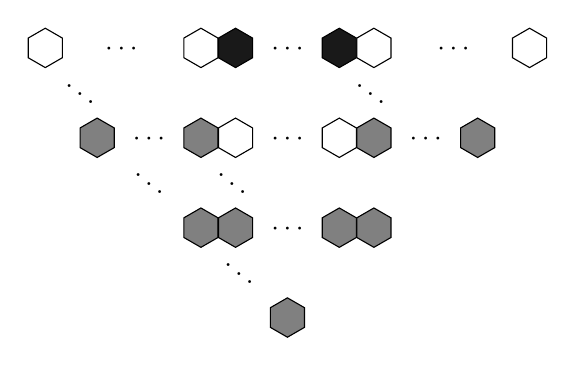
\begin{tikzpicture}[scale=0.25]
  %3^(k'+1)段目
  \filldraw[fill=\myRed,yshift={25*sqrt(3)*5}] (0,0)--++(30:1)--++(90:1)--++(150:1)--++(210:1)--++(270:1)--cycle;
  %3^k'+2 〜 3^(k'+1)-1段目
  \node[xshift={-25*0.7},yshift={25*sqrt(3)*1.85}](0,0){$\ddots$};
  \node[xshift={25*0.7},yshift={25*sqrt(3)*1.85}](0,0){$\iddots$};
  %3^k'+1段目
  \filldraw[fill=\myRed,xshift={-25*5},yshift={25*sqrt(3)*8}] (0,0)--++(30:1)--++(90:1)--++(150:1)--++(210:1)--++(270:1)--cycle;
  \filldraw[fill=\myRed,xshift={-25*3},yshift={25*sqrt(3)*8}] (0,0)--++(30:1)--++(90:1)--++(150:1)--++(210:1)--++(270:1)--cycle;
  \node[yshift={25*sqrt(3)*2.15}](0,0){$\cdots$};
  \filldraw[fill=\myRed,xshift={25*3},yshift={25*sqrt(3)*8}] (0,0)--++(30:1)--++(90:1)--++(150:1)--++(210:1)--++(270:1)--cycle;
  \filldraw[fill=\myRed,xshift={25*5},yshift={25*sqrt(3)*8}] (0,0)--++(30:1)--++(90:1)--++(150:1)--++(210:1)--++(270:1)--cycle;
  %3^k'+1 〜 3^(k'+1)-1段目
  \node[xshift={-25*2},yshift={25*sqrt(3)*2.6}](0,0){$\ddots$};
  \node[xshift={25*0.8},yshift={25*sqrt(3)*2.6}](0,0){$\iddots$};
  \node[xshift={-25*0.8},yshift={25*sqrt(3)*2.6}](0,0){$\ddots$};
  \node[xshift={25*2},yshift={25*sqrt(3)*2.6}](0,0){$\iddots$};
  %3^k'段目
  \filldraw[fill=\myRed,xshift={-25*11},yshift={25*sqrt(3)*11}] (0,0)--++(30:1)--++(90:1)--++(150:1)--++(210:1)--++(270:1)--cycle;
  \node[xshift={-25*2},yshift={25*sqrt(3)*2.9}](0,0){$\cdots$};
  \filldraw[fill=\myRed,xshift={-25*5},yshift={25*sqrt(3)*11}] (0,0)--++(30:1)--++(90:1)--++(150:1)--++(210:1)--++(270:1)--cycle;
  \filldraw[fill=\myYellow,xshift={-25*3},yshift={25*sqrt(3)*11}] (0,0)--++(30:1)--++(90:1)--++(150:1)--++(210:1)--++(270:1)--cycle;
  \node[yshift={25*sqrt(3)*2.9}](0,0){$\cdots$};
  \filldraw[fill=\myYellow,xshift={25*3},yshift={25*sqrt(3)*11}] (0,0)--++(30:1)--++(90:1)--++(150:1)--++(210:1)--++(270:1)--cycle;
  \filldraw[fill=\myRed,xshift={25*5},yshift={25*sqrt(3)*11}] (0,0)--++(30:1)--++(90:1)--++(150:1)--++(210:1)--++(270:1)--cycle;
  \node[xshift={25*2},yshift={25*sqrt(3)*2.9}](0,0){$\cdots$};
  \filldraw[fill=\myRed,xshift={25*11},yshift={25*sqrt(3)*11}] (0,0)--++(30:1)--++(90:1)--++(150:1)--++(210:1)--++(270:1)--cycle;
  %1 〜 3^k'-1段目
  \node[xshift={-25*3},yshift={25*sqrt(3)*3.35}](0,0){$\ddots$};
  \node[xshift={-25*1.2},yshift={25*sqrt(3)*3.35}](0,0){$\iddots$};
  \node[xshift={25*1.2},yshift={25*sqrt(3)*3.35}](0,0){$\ddots$};
  \node[xshift={25*3},yshift={25*sqrt(3)*3.35}](0,0){$\iddots$};
  %0段目
  \filldraw[fill=\myYellow,xshift={-25*14},yshift={25*sqrt(3)*14}] (0,0)--++(30:1)--++(90:1)--++(150:1)--++(210:1)--++(270:1)--cycle;
  \node[xshift={-25*2.4},yshift={25*sqrt(3)*3.65}](0,0){$\cdots$};
  \filldraw[fill=\myYellow,xshift={-25*5},yshift={25*sqrt(3)*14}] (0,0)--++(30:1)--++(90:1)--++(150:1)--++(210:1)--++(270:1)--cycle;
  \filldraw[fill=\myBlue,xshift={-25*3},yshift={25*sqrt(3)*14}] (0,0)--++(30:1)--++(90:1)--++(150:1)--++(210:1)--++(270:1)--cycle;
  \node[yshift={25*sqrt(3)*3.65}](0,0){$\cdots$};
  \filldraw[fill=\myBlue,xshift={25*3},yshift={25*sqrt(3)*14}] (0,0)--++(30:1)--++(90:1)--++(150:1)--++(210:1)--++(270:1)--cycle;
  \filldraw[fill=\myYellow,xshift={25*5},yshift={25*sqrt(3)*14}] (0,0)--++(30:1)--++(90:1)--++(150:1)--++(210:1)--++(270:1)--cycle;
  \node[xshift={25*2.4},yshift={25*sqrt(3)*3.65}](0,0){$\cdots$};
  \filldraw[fill=\myYellow,xshift={25*14},yshift={25*sqrt(3)*14}] (0,0)--++(30:1)--++(90:1)--++(150:1)--++(210:1)--++(270:1)--cycle;
\end{tikzpicture}

      \caption{$n$が奇数 かつ $2 \cdot 3^{k} + 1 \leq n < 3^{k+1}$}
      \label{fig:longodd_steps}
    \end{figure}
\end{itemize}
\newpage

